\documentclass[../main.tex]{subfiles}
%\graphicspath{{\subfix{images/}}}

\begin{document}

\subsection{Motivations}
\paragraph{Why study Lattice-based Cryptography?}
There are a few ways to answer this question.
\begin{enumerate}\itemsep1mm\parskip0mm
 \item It is useful to have cryptosystems that are based on a variety of hard computational problems so the different cryptosystems are not all vulnerable in the same way. 
 \item The computational aspects of lattice-based crytosystems are usually simple to understand and fairly easy to implement in practice.
 \item Lattice-based cryptosystems have lower encryption/decryption computational complexities compared to popular cryptosystems that are based on the integer factorisation or the discrete logarithm problems. 
 \item Lattice-based cryptosystems enjoy strong worst-case hardness security proofs based on approximate versions of known NP-hard lattice problems. % that are conjectured to be hard to approximate
% are (mostly) based on known NP-hard problems % like the Shortest Integer Problem, 
 \item Lattice-based cryptosystems are believed to be good candidates for post-quantum cryptography, since there are currently no known quantum algorithms for solving lattice problems that perform significantly better than the best known classical (non-quantum) algorithms, unlike for integer factorisation and (elliptic curve) discrete logarithm problems
 \item Last but not least, interesting structures in lattice problems have led to significant advances in Homomorphic Encryption, a new research area with wide-ranging applications.
\end{enumerate}

Let’s look at that third point in more details.

Note first that the discrete logarithm and integer factorisation problem classes, which underlie several well-known cryptosystems, are only known to be in NP, they are not known to be NP-complete or NP-hard. The way we understand their complexity is by looking at the average run-time complexity of the current best known (non-polynomial) algorithms for those two problem classes on randomly generated problem instances. Using that heuristic complexity measure, we can show that 
\begin{enumerate}\itemsep1mm\parskip0mm
    \item  there are special instances of those problems that can be solved in polynomial time but, in general, both problems can be solved only in sub-exponential time; and
    \item on average, most of the discrete logarithm and integer factorisation problem instances are as hard as each other.
\end{enumerate} 
So we believe these two problems to be average-case hard problem classes, but we cannot yet prove that. 
Interestingly, we know there are quantum algorithms that can solve these two problems efficiently (\cite{bernstein09}).

The above then begs the question of whether we can design cryptosystems based on known NP-hard or worst-case hard problem classes. %The challenge, of course, is that most NP-hard problem classes are only hard in the worst case but are efficiently solvable on many if not most cases. 
In constructing a (public-key) cryptosystem using a problem class $\mathit{ACH}$ with average-case hardness like Integer Factorisation or Discrete Logarithm, it is sufficient to show that the generation of a key pair (at random) and the solution of the private key corresponds to a problem instance $I \in \mathit{ACH}$, and we rely on average hardness to say $I$ is hard to solve with good probability. But in constructing a (public-key) cryptosystem using a problem class $\mathit{WCH}$ with only known worst-case complexity, we need to do a bit more work, in that it is not sufficient to generate a key pair (at random) and show the solution of the private key is a problem instance $I \in \mathit{WCH}$, we need to actually show that $I$ is one of the hard or worst cases in $\mathit{WCH}$.

In other words, to build a cryptosystem based on a worst-case hard problem class, we do not just need to know that hard instances exist, but we need a way to explicitly generate the hard problem instances. And that is an issue because we do not know how to do that for most worst-case hard problem classes. But this is what makes lattice problems interesting: we know how to generate, through reductions, the worst-case problem instances of approximation versions of NP-hard lattice problems and build efficient crytosystems based on them. In practice, this means breaking these cryptosystems, even with some small non-negligible probability, is provably as hard as solving the underlying lattice problem approximately to within a polynomial factor in polynomial time.

How hard are these approximation lattice problems?
In most cases, the underlying lattice problem is the Shortest Vector Problem (SVP), and the approximation version is called the GapSVP$_{\lambda}$ problem for an approximation factor $\lambda$.
These gap lattice problems are known to be NP-hard only for small approximation factors like $n^{O(1/\log^2 n)}$.
We also know that these gap lattice problems are not NP-hard for approximation factors above $\sqrt{n/\log n}$, unless the polynomial time hierarchy collapses. (See \cite{micciancio-goldwasser02,khot05,khot10} for surveys of these results.)
The best known algorithm (\cite{ajtaiKS01}) for solving these gap lattice problems to within poly(n) factor has time complexity $2^{O(n)}$, which leads us to the following conjecture that underlies the security of lattice-based cryptography:
\begin{quote}
    Conjecture: There is no polynomial time algorithm that approximates lattice problems to within polynomial factors.
\end{quote}

% 

% can show that there are so-called gap versions of known NP-hard problems like the Shortest Vector Problem
% both worst-case hard and we know how to generate those hard problem instances.

% In particular, lattice problems like the Shortest Vector Problem (and related problems) have been proven to be NP Hard under the “randomised reduction hypothesis”, in which the class of polynomial-time algorithms is enlarged to include those that are not deterministic but will, with high probability, terminate in polynomial time with a correct result. And Miklos Ajtai, through his worst-case to average-case reduction technique, show how the hard lattice problem instances can be explicitly generated (through one-way functions). The NP-Hard-ness of these lattice problems is the reason why cryptosystems built on top of them are conjectured to be safe from quantum computing.

% One final word on security. The proof-of-security of lattice-based cryptosystems, like many other cryptosystems, rests on the assumption that $P \neq NP$. This is widely believed to be the case, but the prominent computer scientist Donald Knuth has publicly stated he believes it may be the case that $P = NP$, but that many polynomial algorithms are effectively undiscoverable by us. His intuition is based on several well-known non-constructive proofs of polynomial algorithms, that is, proofs that show the existence of polynomial algorithms for solving certain apparently difficult computational problems for which actual explicit polynomial algorithms are unknown. (The reader is encouraged to take a look at this post and the Knuth interview with Lex Fridman to get more details: https://motls.blogspot.com/2020/01/donald-knuth-clarifies-why-pnp-seems.html). So it may well be that $P = NP$ but the cryptosystems we know and love are still safe because we can only know polynomial algorithms for breaking these cryptosystems exist but we can’t explicitly construct them, and using Marcus Hutter’s Fastest and Shortest Algorithm for All Well-Defined Problems to construct such algorithms will still take way too long in practice…


\paragraph{Why another paper on Lattice Cryptography and Homomorphic Encryption?}
It is important to state early that this tutorial is a compilation of known results in the literature and we do not claim any research originality.
% To make life easier for readers, we have tried to make it as self-contained as possible, with all relevant background given either in the body of the tutorial or in the appendix.
In contrast with \cite{peikert16decade, halevi2017homomorphic, chi15}, this tutorial 
\begin{enumerate}\itemsep1mm\parskip0mm
 \item is written primarily with pedagogical considerations in mind;
 \item is as self-contained as possible, with essentially all required background given either in the body of the tutorial or in the appendix;
 \item focuses mostly on the narrow development path from the Learning With Errors (LWE)\index{LWE} problem to Ring LWE and homomorphic encryption schemes built on top of them; we do not cover other lattice cryptographic systems like NTRU, Ring SIS-based systems, and homomorphic signatures;
 \item provides practical programming examples to help illustrate key concepts throughout the paper. 
\end{enumerate}
The target audience is students, practitioners and researchers who want to learn the "core curriculum" of lattice-based cryptography and homomorphic encryption from a single source. %, but not the research frontiers.

In writing the tutorial, we have benefited from peer-reviewed published papers as well as many less-formal explanatory material in the form of lecture notes and blog articles.
We are not always careful and comprehensive in citing the latter class of material, and we apologise in advance for errors of omission. 



\subsection{Tutorial organisation}

% The mainstream research of lattice-based cryptography is based on lattices that are cyclotomic number fields. Hence, the primary focus of this tutorial paper is to understand the specialities of cyclotomic number fields for producing efficient and secure lattice-based cryptosystems.

\iffalse
The following are the key areas to understand lattice-based cryptography and homomorphic encryption. 
\begin{enumerate}
    \item Group theory - basic group theory concepts and theorems to help understand similar results in ring and field theories, and some well-known groups that will be used later in Galois theory, normal subgroups, equivalence relations, cosets.
    \item Ring theory - in particular polynomial ring, ideal and different kinds of ideals, prime ideal, maximal ideal, quotient ring.
    \item Field theory - finite field, field extension and related.
    \item Algebraic number theory - in particular algebraic number field, cyclotomic polynomial, cyclotomic extension.
    \item Galois theory - Galois group of field extension, Galois extension, minimal polynomial, splitting field, why Galois group is needed in understanding lattice-based cryptography. 
    \item Lattice theory - lattice problems and gap versions of lattice problems, basis, fundamental regions, good and bad basis, LLL, Babai's algorithm, cyclic lattice, ideal lattice.
    \item Computational complexity theory - all the mathematical background mentioned above are essential for designing and proving secure cryptosystems. Some key concepts of computational complexity theory are needed in order to understand what security means in cryptography. Some of the standard and advanced reduction strategies will be used to prove the security of lattice-based cryptosystems. P, NP, polynomial reduction, hardness of approximation, gap problem, gap reduction, search to decision reduction, worst case and average case hardness, average case to worst case reduction, quantum reduction?
\end{enumerate}
\fi

The tutorial can be divided into three parts in pedagogical order as follows. Each part will be presented with definitions, examples, discussions around the intuitions of abstract concepts and more importantly corresponding computer code to help develop the understanding.

After brief introductions to the basics of Computational Complexity Theory in Section~\ref{sec:computational complexity} and Cryptography in Section~\ref{sec:crypto}, the first part of the tutorial focuses on the LWE problem, a foundational hard lattice problem. This part begins with some Lattice Theory in Section~\ref{section:lattice theory}, followed by material on Discrete Gaussian Distributions in Section~\ref{sec:discrete gaussian}.
The LWE problem is then described in some detail in Section~\ref{section:lwe}, including hardness proofs.

% , both are essential in later lattice-based cryptosystems.

The second part discusses the Ring LWE (RLWE) problem, which is a generalization of LWE from the integer domain to an algebraic number field domain that allows more computationally efficient crytosystems to be built. %in order to improve reduce LWE's public key size from roughly quadratic to linear. 
As LWE does not straightforwardly generalize to its ring version, some required background knowledge will be presented with intuition, examples and computer code, including cyclotomic polynomials and their Galois groups in Section~\ref{sec:cyclotomic} and and algebraic number theory in Section~\ref{sec:ant short}.
(For readers that require a more extensive background, the appendix covers Abstract Algebra, Galois Theory and Algebraic Number Theory in significantly more details.)
The RLWE problem is described in some detail in Section~\ref{section:rlwe}, including hardness proofs.
(A mindmap is given in Appendix~\ref{sec:mind maps} to help readers navigate and remember the many components of RLWE proofs.)

Having introduced the LWE and RLWE problems, the final part of the tutorial (Section~\ref{sec:he}) shows how efficient homomorphic encryption (HE) schemes can be developed based on the LWE and RLWE problems.
% aims to develop an intuition of how to design efficient HE schemes based on these hard problems. In particular, the course focuses on a series of works that are considered as the second generation of HE developments. 
These schemes are both similar and different to Gentry's  original fully HE scheme. The similarity is in designing a somewhat HE scheme first, then using bootstrapping to achieve fully HE. The difference is that they avoided using Gentry's ``squashing'' technique, but used the algebraic properties of (R)LWE instances to make the somewhat HE schemes bootstrappable.  


% \subsection{Background}


\subsection{A simple lattice-based encryption scheme}\label{subsec:regev scheme}

Before diving into the technical details of lattice-based cryptosystems and homomorphic encryption schemes, we describe a simple public-key encryption scheme from \cite{regev2009lattices} to illustrate the connection between the scheme's security and lattice problems. This scheme is based on the learning with errors (LWE) problem, see Section \ref{section:lwe} for details. Its simplicity inspired subsequent developments in homomorphic encryption schemes that are based on lattices, and is a fundamental building block in many such schemes. 

Note that in this example $\Z_q$ is the collection of integers in the range $[-q/2, q/2)$.
The parameters  $n,q,N,\chi$ correspond to the vector dimension, the plaintext modulus, the number of LWE samples, and the noise distribution over $\Z_q$, respectively. In particular, $\chi$ is chosen such that $\text{Pr}(|\vc{e} \cdot \vc{r}| < \floor{\frac{q}{2}}/2) > 1 - \text{negl}(n)$ for a random binary vector $\vc{r} =\{0,1\}^N$.
The scheme is summarized as follows, but in an alternative format to be consistent with later homomorphic encryption schemes that will be presented in \Cref{sec:he}.
% Note that all additions in this example are modular additions within the domain $\Z_q = [-q/2,q/2)$. \textcolor{red}{This isn't quite true. We bounce back and forth between values mod $q$, values mod $2$, and integers. It isn't really a problem since we have obvious embedding maps between the various spaces, but we should probably try to be precise about what is really going on.} \kl{You are right, Regev used $Z_q=[0,\dots,q-1]$, Brakerski's schemes used the symmetric range $[-q/2,q/2)$. I saw it in somewhere it's for computational purpose.}
% The scheme is summarized as follows. 

\begin{tcolorbox}
\noindent
\textbf{Private key}: Sample a private key $\vc{s} = (1,\vc{t})$, where $\vc{t} \leftarrow \Z_q^n$.\\

\textbf{Public key}: Sample a random matrix $\vc{A} = \left[\vc{a}_1 \cdots \vc{a}_N\right] \leftarrow \Z_q^{n \times N}$ and compute $\vc{b} = \vc{A}^T \cdot \vc{t} + \vc{e}$ for a random noise vector $\vc{e} \leftarrow \chi^N$. Output the public key $\vc{P}=\sqbracket{\vc{b} \mid -\vc{A}^T} \in \Z_q^{N \times (n+1)}$.\\

\textbf{Encryption:} Encrypt the message $m \in \{0,1\}$ by computing 
\begin{align*}
    \vc{c}=\sqbracket{\vc{P}^T \cdot \vc{r} + \floor{\frac{q}{2}} \cdot \vc{m}}_q \in \Z_q^{n+1},
\end{align*}
where $\vc{m}=(m, 0, \dots, 0)$ has length $n+1$.\\

\textbf{Decryption:} Decrypt the ciphertext $\vc{c}$ using the secret key by computing 
\begin{align*}
    m = \sqbracket{\round{\frac{2}{q}\sqbracket{\vc{c} \cdot \vc{s}}_q}}_2.
\end{align*}
\end{tcolorbox}

\iffalse 
\paragraph{Setup} Given the security parameter $\lambda$, the scheme starts by generating the set of parameters 
\begin{align*}
    \para=(n,q,N,\chi) \leftarrow \setup(1^{\lambda}).
\end{align*}
% that will be used in the following steps. \textcolor{red}{What does the notation $\setup(1^{\lambda})$ mean? In particular, I don't think that $1^{\lambda}$ is meant to indicate exponentiation. It might be useful to define this notation explicitly.} \kl{Good point, I should have defined this properly. In short, the security parameter $\lambda$ corresponds to the running time of the scheme and an adversary's success probability of breaking the scheme. The larger $\lambda$ is, the longer the running time and the smaller the success probability. The notation $1^{\lambda}$ is one way to express the size of $\lambda$ by a string of $\lambda$ ones.} These parameters are inherited from the LWE distribution and are common in all LWE-based schemes \textcolor{red}{We haven't described what the LWE distribution is yet. I don't think we need this sentence at all!} \kl{I was thinking maybe we should briefly introduce LWE?}

% \textcolor{red}{We need to say something about the noise distribution here. Later we claim that the noise has to be small so that the decryption function will work.}.
% In \cite{regev2009lattices}, the author set $q$ to be a prime integer within the range $[n^2, 2n^2]$ and $N=(1+\epsilon)(n+1)\log q$ for an arbitrary constant $\epsilon >0$.
%although the primality requirement of $q$ is not necessary in the LWE distribution setting as we will see later in \Cref{def:lweDist}. \textcolor{red}{While $q$ doesn't have to be prime, it's nice if it is so that we can do the reduction from search to decision problems downstream. Given that, I think it might suffice to just point out what setting Regev used and leave it at that for now.}The LWE sample size was set to $N=(1+\epsilon)(n+1)\log q$ for an arbitrary constant $\epsilon >0$.
%It can also be expressed in a more general form as $N=(n+1)(\log q+O(1))$, which are sometimes used by others. \textcolor{red}{This is another place where I think that striving for generality might muddy the waters a bit. If Regev's values work, then at this point in the paper I don't think we need to also explain what other use too.} \kl{I agree, we don't want give the reader the full details of the scheme, so we should keep it simple and set the parameters as Regev did.}

\paragraph{Key generation} The key generation consists of two parts, the secret key and public key generation.

The secret key generation produces 
\begin{align*}
    \vc{s}=(1,\vc{t}) \leftarrow \seckeygen(n,q),% \text{ where } \vc{t} \leftarrow \Z_q^n 
\end{align*}
where $\vc{t} \leftarrow \Z_q^n$. This key is kept secret and will be used for the decryption of a ciphertext.

% Given the secret key, the public key generation samples a random matrix $\vc{A} = \sqbracket{\vc{a_1} \cdots \vc{a_N}} \leftarrow \Z_q^{n \times N}$ and computes the vector $\vc{b} = \sqbracket{\vc{A}^T \cdot \vc{t} + \vc{e}}_q \in \Z_q^N$ for a random noise vector $\vc{e} \leftarrow \chi^N$. It then treats $\vc{b}$ as a column vector and concatenates it with the negative of the transpose $\vc{A}^T$ to get the public key 
% \begin{align*}
%     \vc{P}=\sqbracket{\vc{b} \mid -\vc{A}^T} \in \Z_q^{N \times (n+1)} \leftarrow \pubkeygen(\vc{t},\para).
% \end{align*}

Given the secret key $\vc{s}$, the public key generation produces
\begin{align*}
    \vc{P}=\sqbracket{\vc{b} \mid -\vc{A}^T} \in \Z_q^{N \times (n+1)} \leftarrow \pubkeygen(\vc{t},\para),
\end{align*}
where $\vc{A} = \sqbracket{\vc{a_1} \cdots \vc{a_N}} \leftarrow \Z_q^{n \times N}$ and ${\vc{b} = \sqbracket{\vc{A}^T \cdot \vc{t} + \vc{e}}_q \in \Z_q^N}$ for a random noise vector $\vc{e} \leftarrow \chi^N$.

% \paragraph{Encryption} To encrypt a message $m \in \{0, 1\}$ by adding it only to the first element of $\vc{P}^T \cdot \vc{r}$, convert the message into a vector $\vc{m}=(m, 0, \dots, 0)$ by appending it with $n$ 0s to the end. Then sample a random binary vector $\vc{r} \leftarrow \Z^N_2$ to compute the following ciphertext 
% \begin{align*}
%     \vc{c}=\sqbracket{\vc{P}^T \cdot \vc{r} + \floor{\frac{q}{2}} \cdot \vc{m}}_q \in \Z_q^{n+1} \leftarrow \enc(\vc{P},m,n,q,N).
% \end{align*}

\paragraph{Encryption} Given the public key $\vc{P}$ and a message $m \in \{0, 1\}$, encryption produces
\begin{align*}
    \vc{c}=\sqbracket{\vc{P}^T \cdot \vc{r} + \floor{\frac{q}{2}} \cdot \vc{m}}_q \in \Z_q^{n+1} \leftarrow \enc(\vc{P},m,n,q,N).
\end{align*}
where $\vc{r} \leftarrow \Z^N_2$ and $\vc{m}=(m, 0, \dots, 0) \in \Z_q^{n+1}$.
% by adding it only to the first element of $\vc{P}^T \cdot \vc{r}$, convert the message into a vector $\vc{m}=(m, 0, \dots, 0)$ by appending it with $n$ 0s to the end. Then sample a random binary vector $\vc{r} \leftarrow \Z^N_2$ to compute the following ciphertext 
\fi 

To demonstrate decryption works, the ciphertext can be re-written as 
\begin{align*}
    \vc{c}=\sqbracket{\vc{b} \cdot \vc{r} + \floor{\frac{q}{2}} \cdot m \mid -\vc{A}^T \cdot \vc{r}}_q,
\end{align*}
%it produces   
%\begin{align*}
 %   m = \sqbracket{\round{\frac{2}{q}\sqbracket{\vc{c} \cdot \vc{s}}_q}}_2. %\leftarrow \dec(\vc{s},\vc{c},q).
%\end{align*}
which implies 
%\noindent{}Notice that
\begin{align*}
    \sqbracket{\vc{c} \cdot \vc{s}}_q
    &= \sqbracket{\vc{b} \cdot \vc{r} + \floor{\frac{q}{2}} \cdot m - \vc{A}^T \cdot \vc{r} \cdot \vc{t}}_q
    = \sqbracket{(\vc{A}^T \cdot \vc{t} + \vc{e}) \cdot \vc{r} + \floor{\frac{q}{2}} \cdot m - \vc{A}^T \cdot \vc{r} \cdot \vc{t}}_q\\
    &=\sqbracket{\vc{e} \cdot \vc{r} + \floor{\frac{q}{2}} \cdot m}_q.
    % &= \sqbracket{\vc{P}^T \cdot \vc{r} + \floor{\frac{q}{2}} \cdot \vc{m}}_q \cdot \vc{s}\\
    % &= \sqbracket{\begin{bmatrix}\vc{b}^T \\ -\vc{A}\end{bmatrix} \cdot \vc{r} + \floor{\frac{q}{2}} \cdot \vc{m}}_q \cdot \vc{s}\\
    %  &= \sqbracket{\begin{bmatrix}\vc{t}^T\vc{A} + \vc{e}^T \\ -\vc{A}\end{bmatrix} \cdot \vc{r} + \floor{\frac{q}{2}} \cdot \vc{m}}_q \cdot \vc{s} \\
     %&= \sqbracket{\begin{bmatrix} \vc{A}^T \cdot \vc{t} \cdot \vc{r} + \vc{e} \cdot \vc{r} \\ -\vc{A}\cdot \vc{r} \end{bmatrix} + \floor{\frac{q}{2}} \cdot \vc{m}}_q \cdot \vc{s},
\end{align*}
%which implies 
%\begin{align*}
%     \sqbracket{\vc{c} \cdot \vc{s}}_q =
    %  \sqbracket{\begin{bmatrix} \vc{t}^T\vc{A}\vc{r} + \vc{e} \cdot \vc{r} \\ -\vc{A}\cdot \vc{r} \end{bmatrix} \cdot \vc{s} + \floor{\frac{q}{2}} \cdot \vc{m} \cdot \vc{s}}_q \\
    %  &= \sqbracket{\begin{bmatrix} \vc{t}^T\vc{A}\vc{r} + \vc{e} \cdot \vc{r} \\ -\vc{A}\cdot \vc{r} \end{bmatrix} \cdot \begin{bmatrix} 1 \\ \vc{t}\end{bmatrix} + \floor{\frac{q}{2}} \cdot \vc{m} \cdot \begin{bmatrix} 1 \\ \vc{t}\end{bmatrix}}_q \\
%     \sqbracket{\vc{e} \cdot \vc{r} + \floor{\frac{q}{2}} \cdot m}_q.
%\end{align*}

\noindent{}Because $\text{Pr}(|\vc{e} \cdot \vc{r}| < \floor{\frac{q}{2}}/2) > 1 - \text{negl}(n)$, we have (with overwhelming probability)
% \begin{equation*}
% \sqbracket{\vc{c} \cdot \vc{s}}_q \in
% \begin{cases}
% (-q/4,q/4) & \text{if $m=0$;} \\
% [-q/2, -q/4) \cup (q/4,q/2) & \text{if $m = 1$}.
% \end{cases}
% \end{equation*}
% Similarly, we have
\begin{equation*}
\frac{2}{q}\sqbracket{\vc{c} \cdot \vc{s}}_q \in
\begin{cases}
(-1/2,1/2) & \text{if $m=0$;} \\
[-1, -1/2) \cup (1/2,1) & \text{if $m = 1$}.
\end{cases}
\end{equation*}
%and
%\begin{equation*}
%    \text{Dec}(\vc{s}, \text{Enc}(\vc{P}, m, n, q, N), q) = \text{Dec}(\vc{s}, \vc{c}, q) = \sqbracket{\left\lfloor\frac{2}{q}\sqbracket{\vc{c} \cdot \vc{s}}_q\right\rceil}_2 = m.
%\end{equation*}

Notice that if $\vc{b}^{\prime} = \vc{A}^T \cdot \vc{t}$ then an attacker who knows $\vc{A}$ and $\vc{b}^{\prime}$ could recover the secret $\vc{t}$ by solving a system of linear equations. The security of the system therefore depends on the presence of the noise vector $\vc{e}$.

If an attacker knows $\vc{b}$ instead of $\vc{b}^{\prime}$, then the attack described above will not work. If, however, such an attacker could recover the noise vector $\vc{e}$, then they could use that information to compute $\vc{b}^{\prime}$. They could then recover $\vc{t}$ as described above. Recovering $\vc{e}$ is an instance of a well-known lattice problem called the bounded distance decoding (BDD) problem. So, an attacker that can solve the BDD problem could recover the secret $\vc{t}$. In other words, recovering $\vc{t}$ is ``no harder'' than solving the BDD problem.

Conversely, in \cite{regev2009lattices} the author showed that the BDD problem is ``no harder'' than recovering $\vc{t}$. That is, an attacker who could recover $\vc{t}$ given $\vc{A}$ and $\vc{b}$ could solve the BDD problem as well. This result implies that if the BDD problem is hard, then attacking the cryptosystem is hard as well. This kind of result is called a \emph{reduction}.
Crucially, the BDD problem is believed to be hard. So, Regev's result constitutes a proof of security for the LWE-based cryptosystem described above.

% \textcolor{red}{MP: I don't think that the following argument quite works with the convention that $Z_q = [q/2, q/2)$. I've replaced it above with one that attempts captures the nuance that comes from the wrapping behaviour.}
% \textcolor{gray}{The first equality is achieved because the noise term has small magnitude. That is, $\text{Pr}(|\vc{e} \cdot \vc{r}| < \floor{\frac{q}{2}}/2) > 1 - \text{negl}(n)$ for the choice of parameters, so $\vc{c} \cdot \vc{s}$ is within modulo $q$. The correctness of the decryption is guaranteed, because when rounding to the next integer, the noise term disappears and the coefficient of the message $m$ rounds to 1 as $q$ is a large integer. 
% Substituting the above into the decryption function then yields 
% \begin{align*}
%     \sqbracket{\round{\frac{2}{q}\sqbracket{\vc{c} \cdot \vc{s}}_q}}_2 
%     = \sqbracket{\round{\frac{2}{q} \bracket{\floor{\frac{q}{2}} \cdot m + \vc{e} \cdot \vc{r}}}}_2
%     = \sqbracket{\round{\frac{2}{q} \floor{\frac{q}{2}} \cdot m + \frac{2}{q} \bracket{\vc{e} \cdot \vc{r}}}}_2.
% \end{align*}
% }
% The security of this scheme is based on the learning with error (LWE) problem \cite{regev05}, which is an average-case problem just like \cite{ajtai1996generating}'s SIS problem, but with more smaller public key size and ciphertext size. The hardness of LWE can be proved using (classical and quantum) reductions from lattice problems as shown in \Cref{fig:lweReduction_intro}. For demonstration purpose, we assume LWE is hard. A sketch of the proof is included in \Cref{subsec:lweHardnessProof}. Next we show that if the above encryption scheme is breakable with non-negligible probability, then the attack can be turned into a mechanism to solve the LWE problem, which contradicts our assumption that it is an average-case hard problem. 

% \begin{figure}[hbt!]
%     \centering
%     \includegraphics[page=14]{images/Lattice_crypto_tikz_folder.pdf}
%     \caption{Reductions to the LWE decision problem. If DGS can be solved for a small scale $r$ close to its lower bound $\sqrt{2n} \eta_{\epsilon}(L)/\alpha$, then both lattice problems can be solved with close to optimal solutions. The key to solve DGS for small $r$ is to iteratively apply a subroutine to gradually reduce the scale. The subroutine supplies discrete Gaussian samples to an LWE oracle to classically solve BDD, the result of which is then used by a quantum algorithm to produce shorter discrete Gaussian samples. \kl{Perhaps simplify the caption for this example.}}
%     \label{fig:lweReduction_intro}
% \end{figure}


% \begin{theorem}
% For any $\epsilon > 0$ and $N \ge (1+\epsilon)(n+1) \log q$, if there exists a polynomial time algorithm $W$ that distinguishes the encryptions of 0 and 1, then there exists a distinguisher $Z$ that distinguishes the LWE distribution $A_{\vc{s},\chi}$ and the uniform distribution $U$ over the same domain for a non-negligible fraction of all possible $\vc{s}$.
% \end{theorem}




\end{document}